\chapter{Experiment and Result}
brief of experiment and result.
\section{Experiment}
Please tell how the experiment conducted from method.

\section{Result}
Please provide the result of experiment

\section{Imron Sumadireja/1164076}
\subsection{Teori}
\begin{enumerate}
\item Klasifikasi Teks dan Gambar Ilustrasi \par
Klasifikasi teks merupakan sebuah model yang digunakan untuk mengkategorikan teks ke dalam kelompok-kelompok yang lebih terorganisir. Jadi untuk setiap kalimat yang di masukan ke dalam mesin, mesin tersebut akan menjadikan setiap kata dari kalimat tersebut menjadi sebuah kolom. Untuk ilustrasinya bisa dilihat pada gambar berikut \ref{Teks1}
		\begin{figure}[ht]
		\centerline{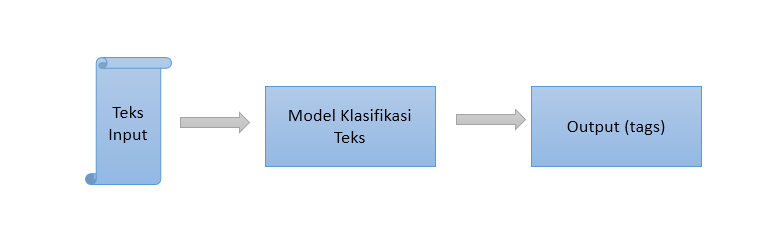
\includegraphics[width=0.5\textwidth]{figures/im/teks1.png}}
		\caption{Klasifikasi teks.}
		\label{Teks1}
		\end{figure}

\item Mengapa klasifikasi bunga tidak bisa menggunakan machine learning \par
Karena machine learning tidak dapat menampilkan inputan sesuai dengan apa yang kita inputkan. Karena inputan tersebut serupa namun mesin memberikan output yang berbeda, biasanya output atau error ini disebut dengan istilah noise. Untuk contoh sederhananya misalkan kita inputkan salah satu label yang terdapat pada bunga, output yang dihasilkan oleh mesin tersebut ialah label yang lain. Itu dikarenakan bunga banyak jenis yang serupa namun tidak sama. Untuk ilustrasinya bisa dilihat pada gambar berikut \ref{Teks2}
		\begin{figure}[ht]
		\centerline{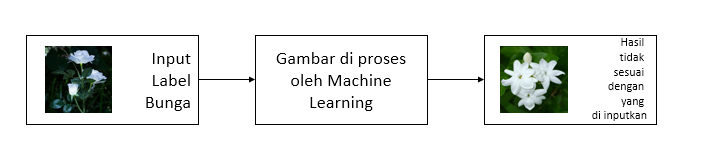
\includegraphics[width=0.5\textwidth]{figures/im/teks2.png}}
		\caption{Klasifikasi Bunga.}
		\label{Teks2}
		\end{figure}

\item Teknik pembelajaran mesin pada untuk kata-kata yang digunakan pada Youtube \par
Teknik yang digunakan pada youtube salah satunya ialah keywords. Dengan keywords tersebut mesin dapat memberikan video sesuai dengan keyword yang kita inputkan pada kolom pencarian. Teknik pembelajarannya tergantung user memberikan input teks seperti apa, karena pada youtube itu sendiri akan menyesuaikan dengan apa yang biasa kita inputkan dan akan memfilter video secara otomatis seuai dengan keyword yang biasa kita inputkan. Contoh ilustrasi sederhananya seperti berikut \ref{Teks3}
		\begin{figure}[ht]
		\centerline{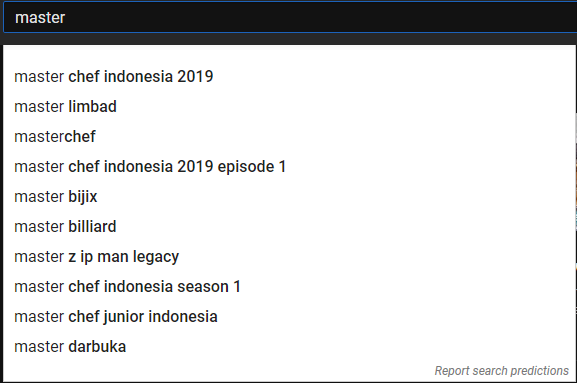
\includegraphics[width=0.5\textwidth]{figures/im/teks3.png}}
		\caption{Klasifikasi teks Youtube.}
		\label{Teks3}
		\end{figure}

\item Vektorisasi data \par
Vektorisasi data merupakan pemecahan atau pembagian data berupa teks, sebagai contoh terdapat 5 paragraf, data teks tersebut di pecah menjadi kalimat-kalimat yang lebih sederhana, lalu di pecah lagi menjadi kata untuk setiap kalimatnya. 

\item Bag of Words \par
Representasi penyederhanaan sebuah kalimat atau perhitungan setiap kata pada suatu kalimat dengan presentase berapa kali muncul kata tersebut untuk setiap kalimatnya. Contoh ilustrasi sederhananya seperti berikut \ref{Teks5}
		\begin{figure}[ht]
		\centerline{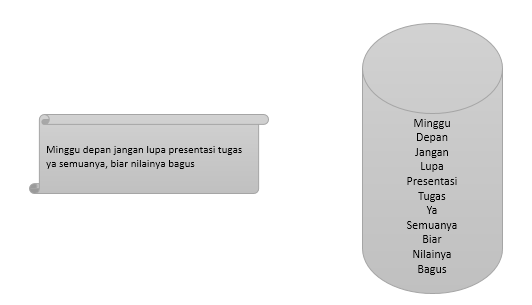
\includegraphics[width=0.5\textwidth]{figures/im/teks5.png}}
		\caption{Bag of Words.}
		\label{Teks5}
		\end{figure}

\item Apa itu TF-IDF \par
TF-IDF merupakan metode untuk menghitung bobot setiap kata pada suatu kalimat yang paling sering digunakan. TF-IDF ini akan menghitung nilai Term Frequency dan Inverse Document Frequency pada setiap kata dalam setiap kalimat yang muncul dengan diimbangi dengan jumlah dokumen dalam korpus yang mengandung kata. Contoh ilustrasi sederhananya seperti gambar berikut \ref{Teks6}
		\begin{figure}[ht]
		\centerline{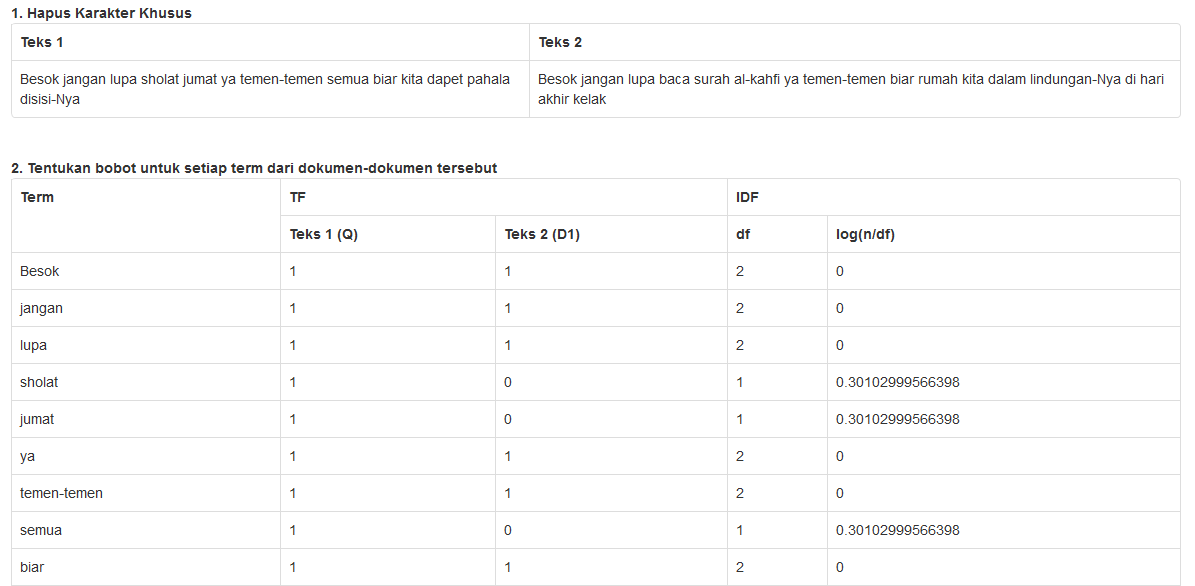
\includegraphics[width=1\textwidth]{figures/im/teks6.png}}
		\caption{TF-IDF.}
		\label{Teks6}
		\end{figure}
\end{enumerate}